


\documentclass[11pt,titlepage,twoside]{report}\usepackage[]{graphicx}\usepackage[table]{xcolor}
% maxwidth is the original width if it is less than linewidth
% otherwise use linewidth (to make sure the graphics do not exceed the margin)
\makeatletter
\def\maxwidth{ %
  \ifdim\Gin@nat@width>\linewidth
    \linewidth
  \else
    \Gin@nat@width
  \fi
}
\makeatother

\definecolor{fgcolor}{rgb}{0.345, 0.345, 0.345}
\newcommand{\hlnum}[1]{\textcolor[rgb]{0.686,0.059,0.569}{#1}}%
\newcommand{\hlsng}[1]{\textcolor[rgb]{0.192,0.494,0.8}{#1}}%
\newcommand{\hlcom}[1]{\textcolor[rgb]{0.678,0.584,0.686}{\textit{#1}}}%
\newcommand{\hlopt}[1]{\textcolor[rgb]{0,0,0}{#1}}%
\newcommand{\hldef}[1]{\textcolor[rgb]{0.345,0.345,0.345}{#1}}%
\newcommand{\hlkwa}[1]{\textcolor[rgb]{0.161,0.373,0.58}{\textbf{#1}}}%
\newcommand{\hlkwb}[1]{\textcolor[rgb]{0.69,0.353,0.396}{#1}}%
\newcommand{\hlkwc}[1]{\textcolor[rgb]{0.333,0.667,0.333}{#1}}%
\newcommand{\hlkwd}[1]{\textcolor[rgb]{0.737,0.353,0.396}{\textbf{#1}}}%
\let\hlipl\hlkwb

\usepackage{framed}
\makeatletter
\newenvironment{kframe}{%
 \def\at@end@of@kframe{}%
 \ifinner\ifhmode%
  \def\at@end@of@kframe{\end{minipage}}%
  \begin{minipage}{\columnwidth}%
 \fi\fi%
 \def\FrameCommand##1{\hskip\@totalleftmargin \hskip-\fboxsep
 \colorbox{shadecolor}{##1}\hskip-\fboxsep
     % There is no \\@totalrightmargin, so:
     \hskip-\linewidth \hskip-\@totalleftmargin \hskip\columnwidth}%
 \MakeFramed {\advance\hsize-\width
   \@totalleftmargin\z@ \linewidth\hsize
   \@setminipage}}%
 {\par\unskip\endMakeFramed%
 \at@end@of@kframe}
\makeatother

\definecolor{shadecolor}{rgb}{.97, .97, .97}
\definecolor{messagecolor}{rgb}{0, 0, 0}
\definecolor{warningcolor}{rgb}{1, 0, 1}
\definecolor{errorcolor}{rgb}{1, 0, 0}
\newenvironment{knitrout}{}{} % an empty environment to be redefined in TeX

\usepackage{alltt}
\usepackage[a4paper, inner=1.5cm, outer=1.5cm, top=2cm, bottom=3cm]{geometry}

\usepackage[utf8]{inputenc} 
\usepackage[T1]{fontenc}
\usepackage[sort&compress]{natbib}
\usepackage[french]{babel}

\addto\captionsfrench{\def\tablename{Tableau}}
\addto\captionsfrench{\renewcommand*{\contentsname}{Sommaire:}}
\addto\captionsfrench{%
  \renewcommand{\listfigurename}{Liste des figures:}%
  \renewcommand{\listtablename}{Liste des tableaux:}%
  \renewcommand{\abstractname}{Résumé}%
}
\usepackage{caption}
\usepackage[labelsep=endash]{caption}
\usepackage{graphicx}
\usepackage{colortbl}
\usepackage{booktabs}
\usepackage{longtable}
\usepackage{array}
\usepackage{multirow}
\usepackage{wrapfig}
\usepackage{float}
\usepackage{pdflscape}
\usepackage{tabu}
\usepackage{threeparttable}
\usepackage{threeparttablex}
\usepackage[normalem]{ulem}
\usepackage{makecell}
\usepackage[table]{xcolor}
\usepackage{ae,aeguill}
\usepackage{subcaption}
\usepackage{textcomp}
\usepackage{hyperref}
\pdfstringdefDisableCommands{%
  \def\\{}%
  }
\hypersetup{ 
colorlinks=true, 
linkcolor=blue, 
citecolor=blue, 
filecolor=blue, 
urlcolor=blue, 
pdftitle= {Suivi des poissons migrateurs sur les STACOMI du bassin de la Seine\\ Année 2023 }, pdfauthor={Sébastien Grall},
pdfsubject={stacomi},
 pdfkeywords={stacomi} {migrateurs} {Seine} {poissons}
}
\pdfoptionpdfminorversion=7
\renewcommand{\sectionmark}[1]{\markboth{}{\emph{\thesection~#1}}}
\renewcommand{\subsectionmark}[1]{\markboth{}{\emph{\thesubsection~#1}}}
\renewcommand{\subsubsectionmark}[1]{\markboth{}{\emph{\thesubsection~#1}}}

\usepackage{fancyhdr}
\pagestyle{fancy}
\fancyhf{}
\rhead{\rightmark}
\lhead{Migration Bassin Seine 2023}
\cfoot{\thepage}
\setlength{\headheight}{15pt}

\usepackage{pdfpages}
\usepackage{setspace}

 %%%%%%%%%%%%%%%%%%%%%%%%%%%%%%%%%%%%%%%%%%%
%%%%%% CHUNK DE CHARGEMENT INITIAL  %%%%%%%
%%%%%%%%%%%%%%%%%%%%%%%%%%%%%%%%%%%%%%%%%%%


%% Makes a path to your graphics' folder.
\graphicspath{{image/}}

\title{Suivi des poissons migrateurs sur les STACOMI du bassin de la Seine,
année 2023}
\IfFileExists{upquote.sty}{\usepackage{upquote}}{}
\begin{document}

\hypersetup{pageanchor=false}

\begin{titlepage}

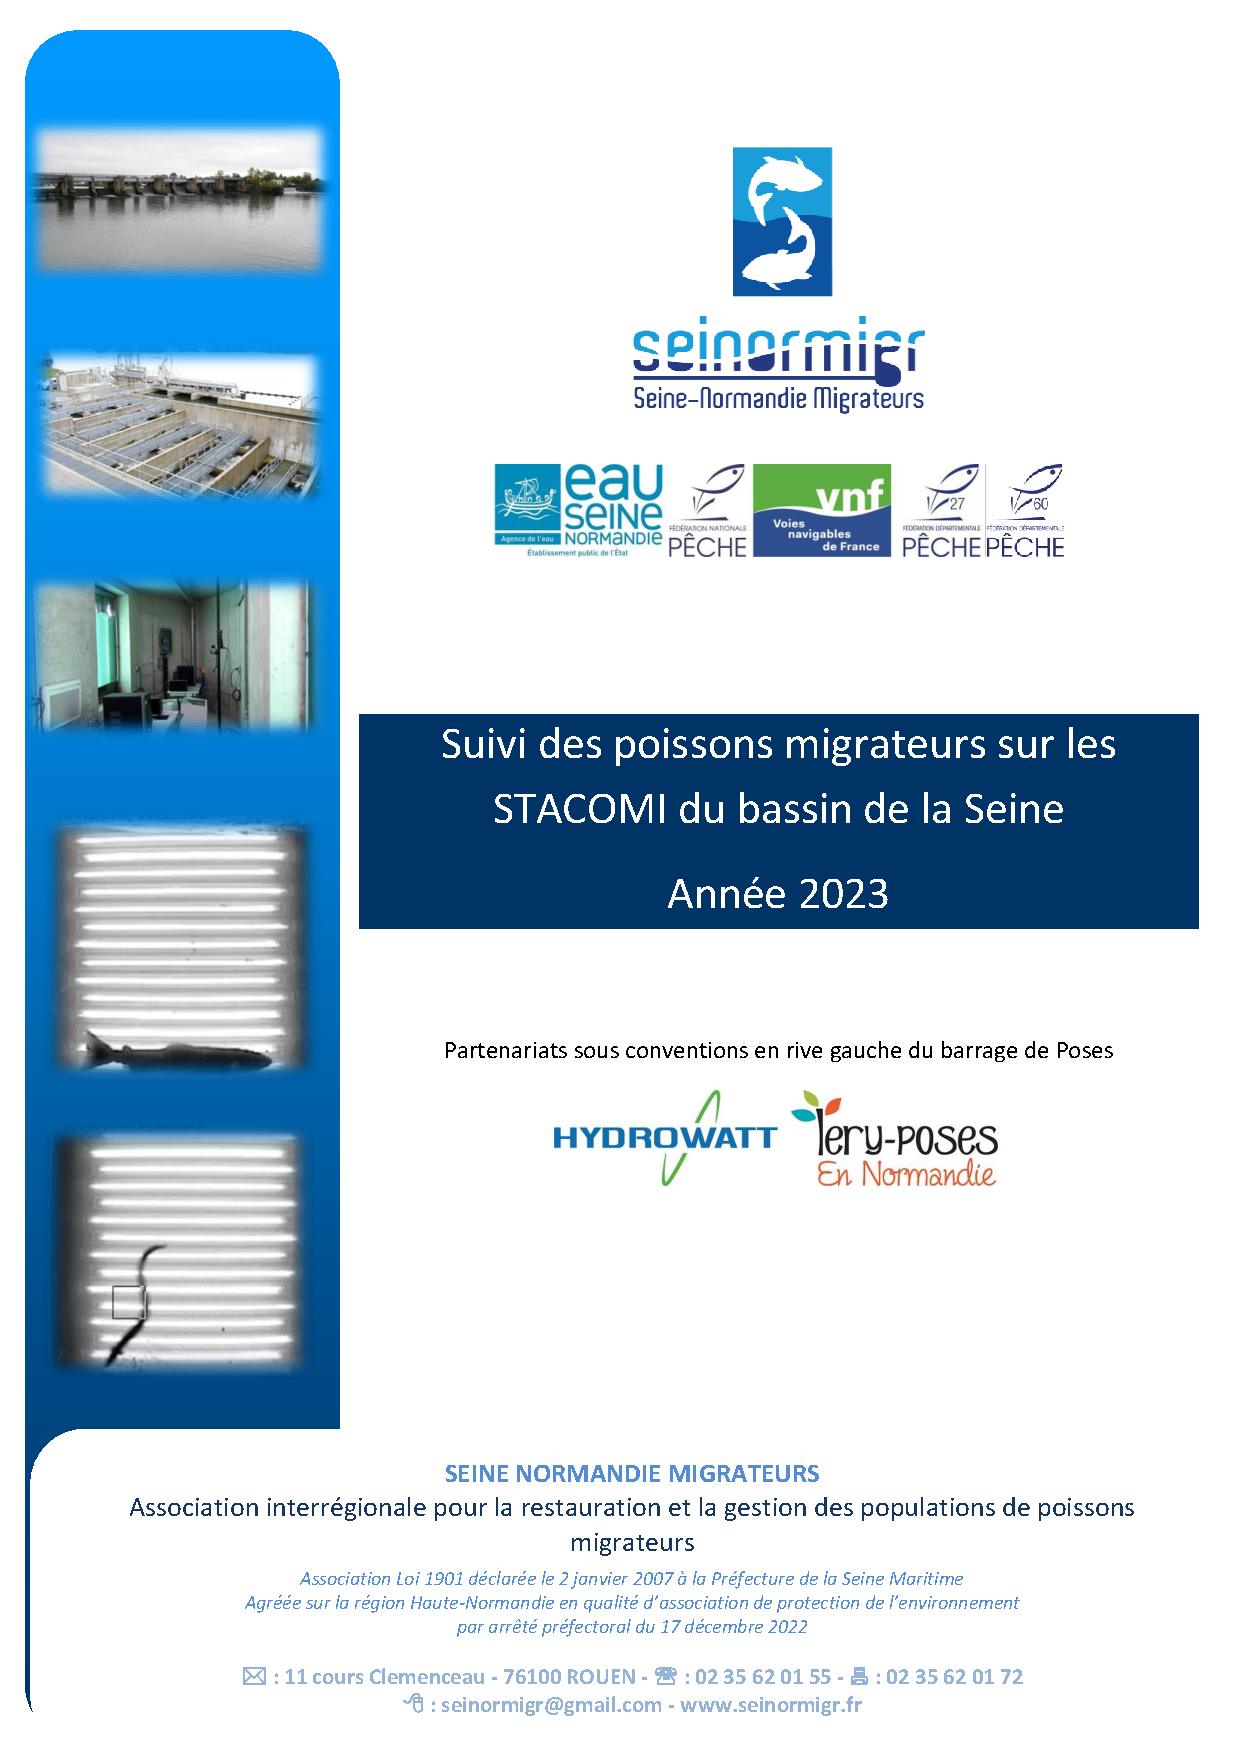
\includepdf[pages=-]{frontpage.pdf}

\end{titlepage}



\newpage
\thispagestyle{empty}
\strut
\newpage

\pagenumbering{roman} \setcounter{page}{1} 

\begin{abstract}

Le résumé

\end{abstract}

\newpage

\tableofcontents

\clearpage

\listoffigures

\listoftables

\hypersetup{pageanchor=false}

\clearpage

\pagenumbering{arabic} \setcounter{page}{1} 



\section{Introduction}

La situation de l'ensemble des poissons migrateurs dans le monde
est similaire : le nombre de populations,
les aires de répartition et les abondances sont en déclin depuis la fin du 19\up{ème} siècle
\citep{saunders_atlantic_1981,bagliniere_reintroductions_1990,parrish_why_2011,jonsson_extinction_1999,
keith_atlas_2001,rochard_identification_2007,limburg_dramatic_2009}.
Le besoin de ces espèces de migrer entre différents habitats essentiels à la finalisation
de leur cycle biologique, implique une vulnérabilité particulière aux perturbations de l'environnement.
Aujourd'hui, la majorité des poissons amphihalins figure dans la liste rouge
des espèces menacées de l'IUCN \citep{limburg_dramatic_2009}.

Sur la Seine, le constat est analogue. Historiquement, 10 espèces amphihalines, dont 8 poissons grands migrateurs
fréquentaient le fleuve sur presque l'ensemble de son bassin versant \citep{moreau_histoire_1881,moreau_les_1898,
poplin_peuplement_1952,euzenat_migren_1992,rochard_identification_2007}, souvent en abondance. Cependant,
en raison d'une anthropisation toujours croissante du fleuve, c'est dès les années 1850 que le déclin s'est amorcé.
Les dégradations sont multiples et semblables à ce qui a été démontré sur d'autres systèmes fluviaux
\citep{nehlsen_pacific_2011,mcdowall_different_1999,lichatowich_depletion_1999,mckinnell_spatial_1999,
limburg_dramatic_2009}. L'édification de barrages, la chenalisation, la pollution, la dégradation des habitats et la surpêche ont conduit au cours du 20\up{ème} siècle à l'extinction des derniers grands migrateurs
\citep{euzenat_migren_1992,belliard_peuplement_1994,mouchel_bassin_1998,boet_multiple_1999,rochard_identification_2007},
seule l'Anguille européenne subsistait encore \citep{boet_multiple_1999,rochard_identification_2007}.

Néanmoins, les efforts entrepris dans le traitement des effluents anthropiques, notamment ceux de l'agglomération parisienne, durant ces deux dernières décennies ont contribué à la franche amélioration de la qualité de l'eau de la Seine \citep{billen_programme_1999,belliard_return_2009,
gousailles_limpact_2009}. Ceci s'est rapidement traduit par le retour des poissons amphihalins, parmi lesquelles deux espèces estuariennes, l'Eperlan (\textit{Osmerus eperlanus}) \citep{pomfret_spatial_1991} et le Flet commun
(\textit{Platichthys flesus}); mais notamment 6 espèces appartenant à la communauté historique des grands poissons
migrateurs de la Seine \citep{rochard_identification_2009} telles que le Saumon atlantique (\textit{Salmo salar}),
la Truite de mer (\textit{Salmo trutta trutta}), la Grande alose (\textit{Alosa alosa}), l'Alose feinte
(\textit{Alosa fallax}) \citep{duhamel_peuplement_2004}, la Lamproie marine (\textit{Petromyzon marinus}) et la
Lamproie fluviatile (\textit{Lampetra fluviatilis}), qui recolonisent peu à peu les parties les plus basses du bassin. L'Anguille européenne (\textit{Anguilla anguilla}) est, quant à elle, présente également sur les zones amonts bien que ses effectifs soient relictuels.

Dès lors, il s'est rapidement avéré primordial de suivre l'évolution de la recolonisation de ces espèces. Pour ce faire, il s'agit de s'intéresser aux éléments clés du cycle biologique liés au domaine continental chaque année. Cela implique
le recensement des zones de frayères et du succès reproducteur; mais avant tout, le dénombrement des géniteurs en montaison en différents points du bassin versant en réponse notamment aux travaux de restauration de la continuité écologique sur le fleuve.

C'est au barrage de Poses dans l'Eure (27), le premier ouvrage sur l'axe Seine, que se sont organisés les premiers éléments de ce suivi, avec la mise en place d'une Station de Contrôle des Migrations (STACOMI) sur la passe à poissons existante en rive gauche depuis octobre 2007. Afin d'assurer la mise en conformité de l'ouvrage dans le cadre du plan de gestion Anguille, le dispositif a été complété en 2013 par l'ajout d'une passe piège à anguilles sur cette même rive.

En raison de la longueur de l'ouvrage (470m) et de la localisation sur le bassin, la rive droite a également été aménagée par les Voies Navigables de France (VNF). Ce nouveau dispositif, mis en service à l'automne 2017 est constitué d'une passe à bassins équipée d'une chambre de vidéo-comptage ainsi qu'une passe piège à anguilles.

Investie depuis plus de 16 ans dans le suivi de la recolonisation du bassin de la Seine par les différentes espèces franchissant à nouveau l'estuaire, Seine-Normandie Migrateurs (Seinormigr) est en charge de l'intégralité des suivi de montaison par vidéo-comptage et par piégeage des anguilles sur le barrage.

Ce rapport présente les résultats des suivis sur les dispositifs de franchissement en rive droite et en rive gauche du barrage de Poses - Amfreville-sous-les-Monts et les associent avec les données historiques afin de donner une vision globale de l'activité migratoire à l'entrée du bassin de la Seine.

\clearpage

\section{Contexte de l'étude}

\clearpage
%\twocolumn
% biblio commune aux différentes années
\bibliographystyle{apalike}
\bibliography{rapport_poses}
\normalsize
\null
\vfill

Rapport Sweave \LaTeX \\
------------------------\\
packages R : \vspace{1mm}
StacomiR \citep{legrand_stacomir_2019}\\
\LaTeX \ :Hmisc, xtable\\
graphiques : ggplot2, cowplot\\
traitements : stringr, lubridate, reshape2, dplyr, plyr, questionr\\
------------------------\\
Dernière compilation : le \today \\
 R version 4.4.1 (2024-06-14 ucrt)\\
 plateforme x86-64-w64-mingw32

\clearpage


\end{document}
